% SQL queries
% Author: SAV

\documentclass[a4paper]{article}
\usepackage[14pt]{extsizes}
\usepackage[utf8]{inputenc}
\usepackage[english,russian]{babel}
\usepackage{amsmath,amsfonts,amssymb,amsthm,mathrsfs,array}
\usepackage{textcomp}
\usepackage{color}
\usepackage{floatflt}
\usepackage{verbatim}
\usepackage{listings}
\usepackage{fancyhdr}
\usepackage{graphicx,picins}
\usepackage[colorlinks]{hyperref}
\usepackage[font=small,labelfont=bf,labelsep=period]{caption} 
\usepackage{tikz}
\usepackage{tkz-euclide}
\usepackage{tikz-3dplot}
\usetikzlibrary{babel,calc,angles,quotes,intersections,through,arrows,shapes,positioning,trees,
				decorations.pathmorphing,decorations.markings}
\usepackage{wasysym}				
\usepackage[width=2.00cm,height=2.00cm,left=1.50cm,right=1.50cm,top=2.00cm,bottom=2.00cm]{geometry}


% ******************** MY commands ********************
													% *
\newtheorem{Def}{Опреление}							% *
\newtheorem{Lem}{Лемма}								% *
\newtheorem{St}{Предложение}						% *
\newtheorem*{Th}{Теорема}							% *
\newtheorem{Con}{Следствие}							% *
\newtheorem{Not}{Замечание}							% *
\newtheorem{Ex}{Пример}								% *
\newtheorem*{Probl}{Задача}							% *
													% *
													% *
\makeatletter										% *
													% *
\renewcommand{\@listi}{								% *
% вертикальные промежутки:							% *
\topsep=0pt % вокруг списка							% *
\parsep=0pt % между абзацами						% *
\itemsep=0pt % между пунктами						% *
% горизонтальные промежутки:						% *
\itemindent=0pt % абзацный выступ					% *
\labelsep=1ex % расстояние до метки					% *
\leftmargin=\parindent % отступ слева				% *
\rightmargin=0pt} % отступ справа					% *
													% *
													% *
\def\th@plain{										% *
	\thm@notefont{}									% *
	%\itshape										% *
}													% *
\newcommand{\MYlvm}{\leavevmode\vspace{-0.3cm}}		% *
\renewcommand{\qedsymbol}{$\blacksquare$}			% *
\newcommand{\MYdef}{\mathrel{\stackrel{\rm def}=}}	% *
													% *
\makeatother										% *
													% *
% *****************************************************




\begin{document}


\begin{flushright}
{\it Groznova Anastasia}
\end{flushright}


\begin{figure}[h]
\noindent\centering{
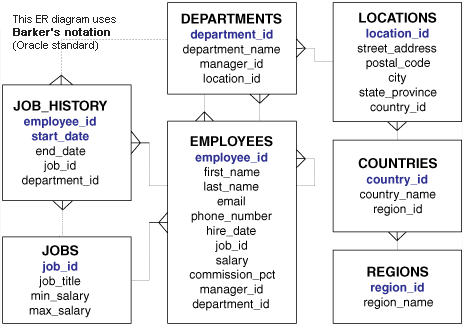
\includegraphics[width=11cm]{EMPLOYEES.png}
}
\caption*{{\bf Рис.~Schema}}
\end{figure}


\noindent
{\large\bf 1.\,Hierarchical queries.}

\vspace{.5cm}
\noindent
{\bf MS-6.1.}
Выведите иерархию подчинений воинских подразделений сверху вниз, начиная с полка 
'Regiment \#1271A', и численность личного состава, приписанного непосредственно к
подразделению. Все подчиненные подразделения должны располагаться "лесенкой" с 
отступом, равным 3-м пробелам. 
О каждом подразделении выводить: название, численность.
\begin{lstlisting}
Regiment #1271A	1
   First Company	1
      Platoon #1	0
      Platoon #2	1
...	...
\end{lstlisting}

\begin{proof}[{\bf Решение.}]\MYlvm\\
\begin{lstlisting} 
SELECT LPAD(' ', 3*(LEVEL-1)) || mu.name AS name, 
( 
    SELECT COUNT(s.person_id) 
    FROM staff s  
    WHERE s.unit_id = mu.unit_id 
) AS count
FROM military_units mu
START WITH name = 'Regiment #1271A'
CONNECT BY PRIOR mu.unit_id = mu.parent_id
\end{lstlisting}
\end{proof}


\noindent
{\bf MS-6.2.}
Выведите иерархию подчинений воинских подразделений сверху вниз, начиная с полка 
'Regiment \#1271A', и численность личного состава, приписанного непосредственно к
подразделению. Все подчиненные подразделения должны располагаться "лесенкой" с 
отступом, равным 3-м пробелам. 
О каждом подразделении выводить: название, численность.
\begin{lstlisting}
Regiment #1271A	1
   First Company	1
      Platoon #1	0
      Platoon #2	1
...	...
\end{lstlisting}
Дополнительное условие~-- НЕ выводить те подразделения~(а также подчиненные им 
подразделения), которые не имеют в составе ни одного военнослужащего.

\begin{proof}[{\bf Решение.}]\MYlvm\\
\begin{lstlisting}
SELECT LPAD(' ', 3*(LEVEL-1)) || name AS name, cnt
FROM 
    ( 
      SELECT 
            mu.unit_id, 
            mu.name, 
            mu.parent_id, 
            count(s.unit_id) AS cnt
      FROM military_units mu 
      LEFT JOIN staff s
      ON mu.unit_id = s.unit_id 
      GROUP BY mu.unit_id, mu.name, mu.parent_id
    )
START WITH name = 'Regiment #1271A' AND cnt > 0
CONNECT BY PRIOR unit_id = parent_id AND cnt > 0
\end{lstlisting}
\end{proof}


\noindent
{\bf MS-6.3.}
Назовем средним сроком службы по подразделению~(таблица military\_units) среднее 
число дней службы на текущий момент всех военнослужащих~(таблица staff), 
приписанных к этому подразделению и ко всем его дочерним подразделениям~ 
(до нижнего уровня). Для каждого из взводов~(military\_units.name начинается с 
'Platoon'), к которым приписаны военнослужащие, вывести имя взвода и средний 
срок службы по взводу, усеченный до дней~(т.е. округленный в меньшую сторону).

\begin{proof}[{\bf Решение.}]\MYlvm\\
\begin{lstlisting}
SELECT 
      tt.name, 
      TRUNC(AVG(TO_DATE(SYSDATE)-TO_DATE(tt.consc_date))) AS p
FROM
    ( 
      SELECT CONNECT_BY_ROOT t.name as name, t.consc_date
      FROM
          ( 
            SELECT mu.*, s.consc_date
            FROM military_units mu 
            LEFT JOIN staff s 
            ON mu.unit_id = s.unit_id 
          ) t
      START WITH t.name LIKE 'Platoon%'
      CONNECT BY PRIOR t.unit_id = t.parent_id 
    ) tt
GROUP BY tt.name
HAVING COUNT(tt.consc_date) > 0
\end{lstlisting}
\end{proof}


\noindent
{\bf MS-6.4.}
Назовем средним сроком службы по подразделению среднее число дней службы на 
текущий момент всех военнослужащих, приписанных к этому подразделению и ко всем 
его дочерним подразделениям~(до нижнего уровня).
Вывести название самого "старшего" подразделения, а также средний срок службы по
подразделению, округленный до дней. В случае, если таких подразделений более 
одного, ограничить вывод первым. \\
Примечание. Эту задачу можно решить по аналогии с задачей {\bf MS-6.3}, но типичная 
ошибка усреднения в {\bf MS-6.3} не влияет на результат, а в данной задаче~-- влияет.

\begin{proof}[{\bf Решение.}]\MYlvm\\
\begin{lstlisting}
SELECT name, period
FROM 
    (
      SELECT 
            tt.name AS name, 
            TRUNC(AVG(TO_DATE(SYSDATE)-TO_DATE(tt.consc_date))) 
            AS period
      FROM
          ( 
            SELECT CONNECT_BY_ROOT t.name AS name, t.consc_date
            FROM
                ( 
                  SELECT mu.*, s.consc_date
                  FROM military_units mu 
                  LEFT JOIN staff s 
                  ON mu.unit_id = s.unit_id 
                ) t
            START WITH t.name LIKE 'Platoon%'
            CONNECT BY PRIOR t.unit_id = t.parent_id 
          ) tt
      GROUP BY tt.name
      HAVING COUNT(tt.consc_date) > 0
      ORDER BY period DESC
    )
WHERE ROWNUM = 1
\end{lstlisting}
\end{proof}


\noindent
{\bf MS-6.5.}
Для каждого военнослужащего званием ниже лейтенанта вывести начальника роты~ 
(подразделения с названием 'Company'), к которой приписан данный военнослужащий.
В обоих столбцах выводить атрибут name.
Примечание: отношение званий~(выше/ниже) хранится в атрибуте priority таблицы 
ranks. Для проверки можно использовать тот факт, что начальник роты является 
майором.

\begin{proof}[{\bf Решение.}]\MYlvm\\
\begin{lstlisting}
SELECT sname, CONNECT_BY_ROOT sname AS boss
FROM
    (
    SELECT 
          s.name AS sname, 
          s.person_id AS pid,
          s.chief AS chief,
          r.name AS rname,
          r.priority AS pr      
    FROM ranks r 
    INNER JOIN staff s 
    ON r.rank_id = s.rank_id
    INNER JOIN military_units mu
    ON s.unit_id = mu.unit_id
    WHERE r.rank_id = s.rank_id 
    ) 
WHERE pr < 5
START WITH rname = 'Major'
CONNECT BY PRIOR pid = chief 
\end{lstlisting}
\end{proof}


\noindent
{\bf MS-6.6.}
Вывести название самого малочисленного взвода~(взвод~-- это подразделение, 
название которого начинается с 'Platoon') и его численность.
При подсчетах численности следует учитывать состав подразделений~(отделений), 
подчиненных данному взводу. Если во взводе нет ни одного военнослужащего, 
он выводиться не должен.

\begin{proof}[{\bf Решение.}]\MYlvm\\
\begin{lstlisting}
SELECT name, cnt
FROM
    (
      SELECT muname AS name, COUNT(pid) AS cnt
      FROM   
          ( 
            SELECT 
                  CONNECT_BY_ROOT mu.name AS muname, 
                  s.person_id AS pid
            FROM staff s, military_units mu  
            WHERE s.unit_id = mu.unit_id 
            START WITH mu.name LIKE 'Platoon%'
            CONNECT BY PRIOR mu.unit_id = mu.parent_id
          ) 
      GROUP BY muname
      ORDER BY cnt
    ) 
WHERE ROWNUM  = 1
\end{lstlisting}
\end{proof}


\noindent
{\bf MS-6.7.}
Для военнослужащего с именем "Vasiliev" вывести всех его подчиненных~(прямых и 
непрямых), у которых, в свою очередь, нет собственных подчиненных. 
Подчинение определяется колонкой chief в таблице staff. \\
Вывод: имя военнослужащего, его звание, название подразделения и ID 
военнослужащего.

\begin{proof}[{\bf Решение.}]\MYlvm\\
\begin{lstlisting}
SELECT sname, rname, sunit, pid
FROM 
    (
      SELECT 
            s.unit_id AS sunit,
            s.name AS sname, 
            s.person_id AS pid,
            s.chief AS chief,
            r.name AS rname, 
            mu.name AS muname 
      FROM ranks r 
      INNER JOIN staff s 
      ON r.rank_id = s.rank_id
      INNER JOIN military_units mu
      ON s.unit_id = mu.unit_id
      WHERE r.rank_id = s.rank_id
    ) t
WHERE CONNECT_BY_ISLEAF = 1
START WITH t.sname = 'Vasiliev'
CONNECT BY PRIOR t.pid = t.chief
\end{lstlisting}
\end{proof}


\noindent
{\bf MS-6.8.}
Перечислить в одной строчке через запятую~(без пробелов) весь личный состав 
первого отделения~(т.е. подразделения с именем 'Squad \#1'), упорядочив там имена
военнослужащих~(name) по алфавиту. \\
Учитывать только военнослужащих, приписанных непосредственно к отделению.

\begin{proof}[{\bf Решение.}]\MYlvm\\
\begin{lstlisting}
SELECT LTRIM(SYS_CONNECT_BY_PATH(name, ','), ',') AS list
FROM 
    ( 
      SELECT ROWNUM r, name 
      FROM 
          (
            SELECT s.name AS name 
            FROM staff s, military_units mu
            WHERE s.unit_id = mu.unit_id AND 
            mu.name = 'Squad #1'
            ORDER BY s.name 
          )
    ) 
WHERE CONNECT_BY_ISLEAF = 1
START WITH r = 1
CONNECT BY r = PRIOR r + 1
\end{lstlisting}
\end{proof}


\noindent
{\bf MS-6.8*.}
Для каждого отделения~(отделение~-- это подразделение, название которого 
начинается со слова 'Squad') перечислить через запятую в одной строчке весь 
личный состав, упорядочив военнослужащих по алфавиту. 
Учитывать только военнослужащих, приписанных непосредственно к отделению.
Вывод: первой колонкой~-- ID подразделения, второй~-- список имен 
военнослужащих~(name) через запятую~(без пробелов).

\begin{proof}[{\bf Решение.}]\MYlvm\\
\begin{lstlisting}
SELECT 
      muname "Unit name", 
      LISTAGG(sname, ',') 
      WITHIN GROUP (ORDER BY muname) "List"
FROM
    (
      SELECT 
            mu.name AS muname, 
            s.name AS sname, 
            s.unit_id AS unit
      FROM military_units mu LEFT JOIN staff s
      ON mu.unit_id = s.unit_id 
      WHERE mu.name LIKE 'Squad%'
    )
GROUP BY muname 
\end{lstlisting}
\end{proof}


\noindent
{\bf MS-6.9.}
Вывести, какие уникальные иерархии подчинения~(от самого старшего командира до 
младшего подчиненного) присутствуют в таблице staff.
Под элементом иерархии понимаются не имя военнослужащего, а его воинское звание~ 
(таблица ranks). Элементы разделяются символом ">", а упорядочиваются от 
старшего к младшему. Например: Colonel>Major>Leutenant>Sergeant

\begin{proof}[{\bf Решение.}]\MYlvm\\
\begin{lstlisting}
SELECT 
      DISTINCT LTRIM(SYS_CONNECT_BY_PATH(r.name, '>'), '>') 
FROM ranks r, staff s
WHERE r.rank_id = s.rank_id AND 
CONNECT_BY_ISLEAF = 1 
START WITH r.name = 'Colonel'
CONNECT BY PRIOR s.person_id = s.chief 
\end{lstlisting}
\end{proof}




\newpage




\noindent
{\large\bf 2.\,Analytical functions.}

\vspace{.5cm}
\noindent
{\bf 7-04.}
Для всех сотрудников вывести id отдела, фамилию, специальность~(job\_id) и 
количество людей в данном отделе с такой специальностью.

\begin{proof}[{\bf Решение.}]\MYlvm\\
\begin{lstlisting}
SELECT 
      department_id, 
      last_name, 
      job_id,
      COUNT(job_id) OVER(PARTITION BY department_id) AS count
FROM employees
\end{lstlisting}
\end{proof}


\noindent
{\bf 7-05.}
Для всех сотрудников вывести фамилию, зарплату, фамилию менеджера и максимальную
зарплату среди непосредственных подчиненных этого менеджера.
Если у сотрудника менеджер отсутствует, никакой информации для такого сотрудника
выводить не нужно.

\begin{proof}[{\bf Решение.}]\MYlvm\\
\begin{lstlisting}
SELECT 
      e.last_name, 
      e.salary, 
      m.last_name, 
      MAX(e.salary) OVER(PARTITION BY m.last_name) AS max
FROM employees e, employees m
WHERE e.manager_id = m.employee_id
\end{lstlisting}
\end{proof}


\noindent
{\bf 7-06.}
Для каждой локации~(таблица LOCATIONS) вывести location\_id, postal\_code и количество локаций с тем же количеством символов в postal\_code.

\begin{proof}[{\bf Решение.}]\MYlvm\\
\begin{lstlisting}
SELECT lid, pc, COUNT(len) OVER(PARTITION BY len) AS cnt
FROM
    (
      SELECT 
            location_id AS lid, 
            postal_code AS pc, 
            LENGTH(postal_code) AS len
      FROM locations
    )
\end{lstlisting}
\end{proof}


\noindent
{\bf 7-09.}
Для каждого сотрудника вывести id отдела, фамилию, дату приема на работу и 
фамилию сотрудника, принятого на работу в этот отдел самым первым. 
Если таких несколько~(приняты в один день)~-- вывести фамилию первого из них. 
Указание: «первый» определяется функцией first\_value.

\begin{proof}[{\bf Решение.}]\MYlvm\\
\begin{lstlisting}
SELECT 
      department_id, 
      last_name, 
      hire_date, 
      FIRST_VALUE(last_name)
        OVER(PARTITION BY department_id ORDER BY hire_date)
FROM employees
\end{lstlisting}
\end{proof}


\noindent
{\bf 7-11.}
Для всех сотрудников вывести отдел (department\_id), фамилию (last\_name), 
зарплату~(salary) и количество человек, которые, работая в этом же отделе, имеют зарплату~(строго) больше, чем данный 
сотрудник.

\begin{proof}[{\bf Решение.}]\MYlvm\\
\begin{lstlisting}
SELECT 
      department_id, 
      last_name, 
      salary, 
      COUNT(*) 
        OVER(PARTITION BY department_id ORDER BY salary 
          RANGE BETWEEN 1 FOLLOWING AND UNBOUNDED FOLLOWING) 
FROM employees
\end{lstlisting}
\end{proof}




\end{document}
